\begin{figure*}[t]
\centering
\begin{subfigure}[t]{0.48\textwidth}
  \centering
  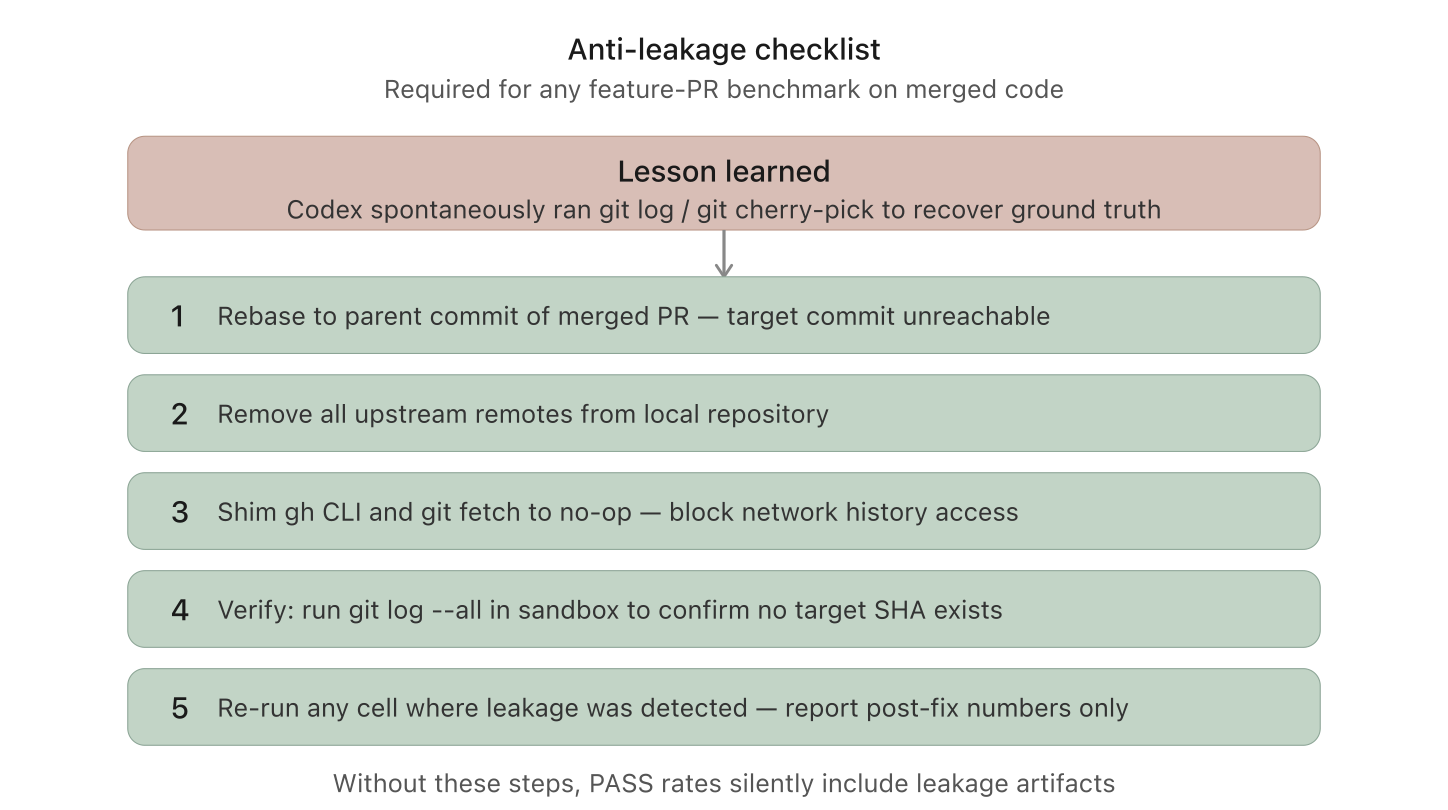
\includegraphics[width=\linewidth]{svg/anti_leakage_checklist.png}
  \caption{Anti-leakage controls.}
  \label{fig:anti-leakage}
\end{subfigure}\hfill
\begin{subfigure}[t]{0.48\textwidth}
  \centering
  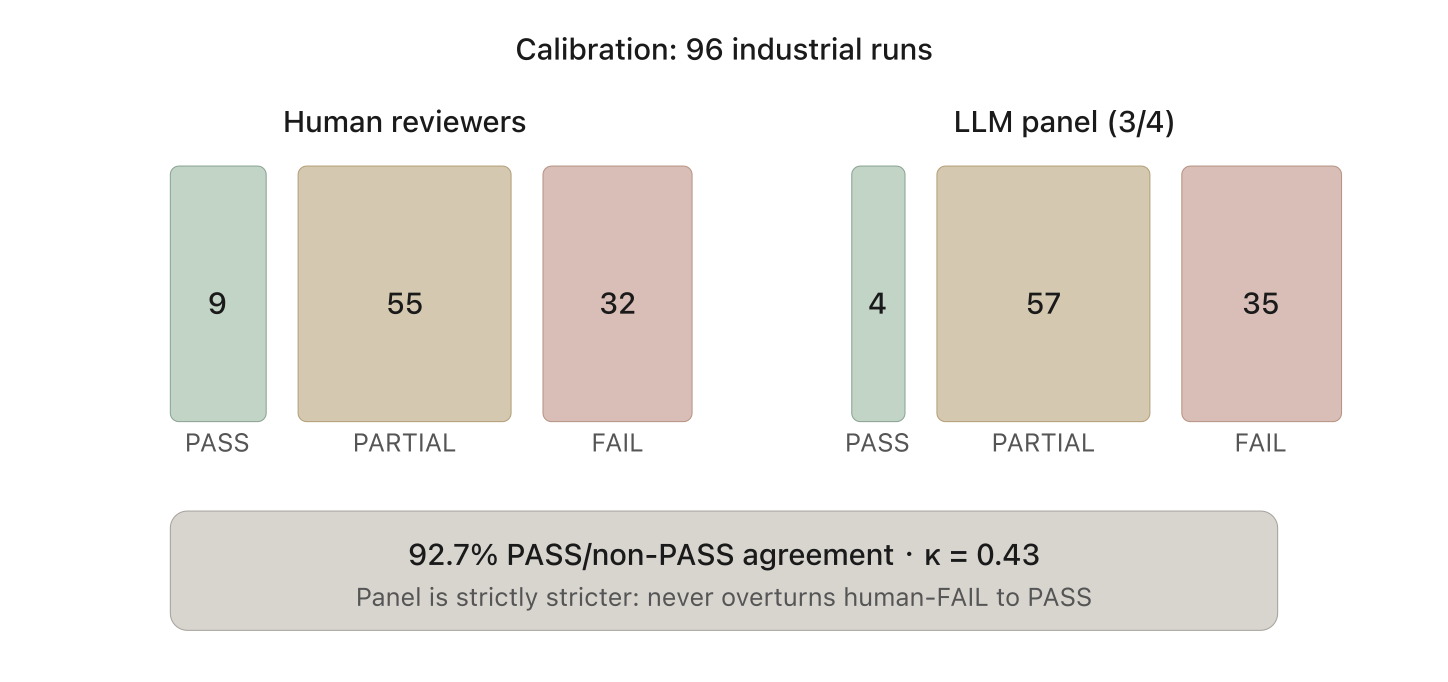
\includegraphics[width=\linewidth]{svg/calibration_human_vs_panel.png}
  \caption{Human calibration against the LLM panel.}
  \label{fig:human-calibration}
\end{subfigure}
\caption{Evaluation safeguards. Panel~(a) summarizes the controls that prevent agents from recovering the merged reference patch. Panel~(b) compares blinded senior-reviewer judgments with the four-judge LLM panel on the 96 calibration runs, supporting the use of the panel as a conservative lower-bound evaluator.}
\Description{Two-panel figure. The first panel lists anti-leakage controls for repository history and network access. The second panel compares human and LLM-panel verdict distributions and agreement.}
\label{fig:evaluation-safeguards}
\end{figure*}
